\documentclass[a4paper, 11pt]{scrartcl}

\usepackage[utf8]{inputenc} % gestion des accents (source)
\usepackage[T1]{fontenc} % gestion des accents (PDF)
%\usepackage[francais]{babel} % gestion du français
\usepackage[english]{babel} % gestion du français
\usepackage{textcomp} % caractères additionnels
\usepackage{xcolor}
\usepackage{caption}
\usepackage{subcaption}
\usepackage{lmodern} % police de caractères
\usepackage{float}
\newcommand{\jump}{\vspace{0.3cm}}

\usepackage[bookmarks=true]{hyperref} % liens hypertexte
\hypersetup{
  colorlinks,
  citecolor=violet,
  linkcolor=black,
  urlcolor=blue}
%\usepackage{pstricks} % encadrage

\usepackage{graphicx}
\usepackage{caption}
\usepackage{amsmath, amsfonts, amssymb}
%\usepackage{listings}
%\usepackage[fancysections]{polytechnique}
\usepackage{fancyhdr}
\usepackage{eso-pic,xcolor,graphicx}
\definecolor{light-gray}{gray}{0.7}

\pagestyle{fancy}
%\usepackage[top=1in, bottom=1.25in, left=1in, right=1in]{geometry}

%\lhead{Convex Neural Networks} 
%\chead{\today}
%\rhead{Eloïse \textsc{Berthier}}

\newtheorem{theorem}{Theorem}[section]
\newtheorem{definition}{Definition}[section]
\newtheorem{proposition}{Proposition}[section]
\newtheorem{corollary}{Corollary}[theorem]
\newtheorem{lemma}[theorem]{Lemma}

\title{On Convex Neural Networks}
\author{Eloïse Berthier}
\date{\today}
\subtitle{Mathematical Foundations of Data Science}


\begin{document}

\setcounter{secnumdepth}{3}
\setlength{\parindent}{0cm}

%\vspace{5em}
\maketitle
%\fontfamily{lmss}\selectfont

\everymath{\displaystyle}

\vspace{12em}

\abstract{Training a neural network is a non convex problem and in general gradient descent algorithms only return local minima. Hence it may yield non reproductible results. One can formulate the empirical risk minimization as a convex problem for one-hidden layer neural networks with infinitely many hidden units. When properly penalized, these neural networks have strong generalization properties and are adaptive to structure on the data. However, optimizing in infinite dimension in hard and for instance the conditional gradient algorithm has a non-polynomial complexity. We follow a recent approach from optimal transport which provides global optimality guarantees for the gradient descent algorithms in the case of overparametrized neural networks, under simple conditions on the initialization. We provide numerical experiments to visualize this phenomenon and to study the overparametrization regime and the influence of the initialization.

\newpage

%\tableofcontents
%\newpage

\section{Introduction}

While the use of neural networks has dramatically increased the performance of some recognition systems, there still lacks a clear mathematical understanding of this success. One of the key issues is that optimizing neural networks is a non-convex problem, hence training algorithms may not return a global minimum.

Yet in practice, training large neural networks often results in satisfying solutions, which are empirically considered \textit{not too far} from a global minimum. Thus it suggests that there may be some implicit assumptions on the data or on the model that are usually verified and could explain this regularity, somehow making the problem \textit{more convex} than at first sight.\\

There have been several attempts to study this phenomenon, heading in different directions. Here are some examples.

Some rely on convex relaxations of the original optimization problem. \cite{zhang2016convexified} define a convex relaxation for training convolutional neural networks. They show that in the case of a two-layer CNN, the generalization error of the solution to the convex relaxed problem converges to that of the best possible two-layer CNN.

In \cite{haeffele2017global} are studied conditions under which the optimization landscape for the non-convex optimization problem is such that all critical points are either global minimizers or saddle points. \cite{visualloss} provide a tool to visualize the loss surface along random directions near the optimal parameters.

There is also a series of some very recent contributions on the problem: \cite{du2018agradient}, \cite{du2018bgradient} and \cite{zou2018stochastic}. They rely on the analysis of the dynamics of the prediction space rather than of the parameter space, the former being governed by the spectral property of a Gram matrix. If the data is \textit{not degenerate}, this Gram matrix’s least eigenvalue is lower bounded, and randomly initialized gradient descent linearly converges to a global optimum.

In the infinite-width limit, \cite{jacot2018neural} relate the evolution of a neural network function to a kernel that they call the \textit{neural tangent kernel}. Convergence to a global minimum can then be related to the positive-definiteness of the limiting kernel, and which is the case when the data is on a sphere.

However, \cite{chizat:hal-01945578} notice that part of these results may be explained by a specific \textit{lazy} training setting which does not reflect practical deep learning applications. \\

In this report, we concentrate on another approach called \textit{convex neural networks}. The core idea was introduced by \cite{bengio2006convex} and focuses on one hidden-layer neural networks. Instead of optimizing the weights of a network with a fixed number of hidden units, we could consider the equivalent problem of optimizing on the set of all the possible hidden unit functions. The training problem is convex with respect to the parameters of the model (which are now only the ouput weights).

Of course, while this approach solves the non-convexity issue, it introduces some other difficulties. These are extensively studied in \cite{bach2017breaking}, on which we will mainly focus in this report. A complete analysis of the generalization performance of convex neural networks is derived, in particular showing that high-dimensional non-linear variable selection may be achieved, without any strong assumption regarding the data. Yet this approach requires to solve a convex problem in infinite dimension and is only possible if the non-convex subproblem of adding a new hidden unit can be solved efficiently. Finding a polynomial-time algorithm approximating well this subproblem induced by the conditional gradient method is still an open question.

\cite{chizat2018global} focus on solving the same convex problem, but avoid the potentially NP-hard problem of optimizing with conditional gradient. Instead, they discretize the unknown measure as a mixture of particles. This approach is inspired by optimal transport and brings strong asymptotical global optimality guarantees for gradient flow optimization. It also provides simple numerical experiments.\\

Looking at all these different approaches, we may notice some recurrent patterns in the assumptions that are commonly made:

\begin{itemize}
\item \textit{one hidden-layer models}: most of the articles focus on simple neural network models, that already include a wide variety of classical supervised learning configurations, but do not directly cover deep neural networks.
\item \textit{over parametrization}: all the good generalization properties are derived in the case of an over parametrized model, yet the key question is \textit{how much} over parametrization is needed.
\item \textit{positive homogeneity}: most of the results are achieved in the case of positively homogeneous activation functions. It could explain the experimental advantage of using ReLU functions over others in deep learning.
\item \textit{proper initialization}: several articles rely on the conservation of an initial regularity through the optimizing process, for instance using gradient flows, and so emphasize the role of the initialization.
\end{itemize}

\section{Towards a Convex Problem}

\subsection{General layout}

We consider single hidden-layer neural networks. It defines a class of prediction functions on $\mathbb{R}^d$ parametrized as: $f_{w, v, b}(x) =\sum_{j=1}^k w_j \sigma(v_j^\top x + b_j)$, where $\sigma$ is a fixed activation function, $k$ is the number of hidden units, $v_j$ and $b_j$ are the weight and bias of layer $j$ and $(w_j)_{j=1,...,k}$ the weights of the output layer. We can eliminate the $b_j$ by integrating it into $v_j$ and adding a one on top of $x$.\\

We will mainly consider a fixed non-decreasing and positively homogeneous  activation function of some integer degree, i.e. $\sigma(u) = (u)^\alpha_+$, for some $\alpha \in \mathbb{N}$ (it includes ReLU and hard-thresolding functions). We will also later consider sigmoid activation functions in the numerical experiments.

\subsection{From non-convexity to convexity}

For a fixed value of $k$, training a neural network is an empirical risk minimization problem: $\min_{w, v} \frac{1}{n} \sum_{i=1}^n \ell(f_{w, v}(x_i), y_i) + \Omega(w, v)$, where $\ell$ is a smooth convex loss function (convex in its first argument) and $\Omega$ a convex regularization function, and $(x_i, y_i)$ the observations in $\mathcal{X} \times \mathbb{R}$. This is not a convex problem because of the non-convexity of the prediction function.\\

Now consider the set $\mathcal{F}_\mathcal{V}$ of all the possible hidden unit functions $\varphi_v : \mathcal{X} \rightarrow \mathbb{R}$, with $\mathcal{X}$ any measurable space. We will call it the set of basis functions. It is parametrized by the compact topological space $\mathcal{V}$ of all possible hidden unit weight vectors. We assume that for all $x \in \mathcal{X}$, the functions $v \mapsto \varphi_v(x)$ are continuous. To represent any affine function, $\mathcal{V}$ has dimension $d + 1$ for inputs in $\mathcal{X}$ of dimension $d$.

Let $\mathcal{W}$ be the Hilbert space of functions from $\mathcal{F}_\mathcal{V}$ to $\mathbb{R}$, with $\cdot$ an inner product. For any $x \in \mathcal{X}$, we define $h(x)$ as the function that maps any $\varphi_v \in \mathcal{F}_\mathcal{V}$ to $\varphi_v(x)$. $h(x)$ is an element of $\mathcal{W}$. $h(x)$ can be seen as the vector of activations of the hidden units when we observe $x$ as input. An element $w$ of $\mathcal{W}$ can also be understood as the output weights vector in a neural network. We extend the definition of $\Omega$ to be a convex regularization functional from $\mathcal{W}$ to $\mathbb{R}$.  \\

We can define the following problem:
\begin{equation}
\min_{w \in \mathcal{W}} \mathcal{C}(w) := \frac{1}{n} \sum_{i=1}^n \ell(w \cdot h(x_i), y_i) + \Omega(w)
\end{equation}

\begin{lemma}
Problem (1) is a convex minimization problem.
\end{lemma}
The proof is straightforward: any Hilbert space $\mathcal{W}$ is convex, $ \ell(w \cdot h(x_i), y_i)$ is convex in $w$ and by additivity the objective function also is.\\

This problem formulation is from \cite{bengio2006convex}. It is a bit hard to handle as it introduces many notations that are not all explicit. Still it provides an intuitive idea of the problem we want to define: considering all the possible hidden units we could pick, how to combine them to make a good prediction, that is, how to choose the output weight $w$ to minimize $\mathcal{C}$. 

In this problem the penalization term is crucial. Unlike the initial optimization problem where the number of hidden units was fixed, it is now part of the optimization problem. Without any regularization, the solution could have an arbitrary large number (possibly infinite) of non-zero variables $w_j$. We will later see that a proper regularization can ensure a finite number of selected units, and so a finite model.

$\mathcal{W}$ is the space of the output weights, and since it has infinite dimension, it is handled as a space of functions. What makes it a bit entangled is that eventually $\mathcal{W}$ is defined as a space of functions (output layer) of functions (hidden layer) of $x\in \mathcal{X}$, but it can also be seen as a simple vector (in potentially infinite dimension). The vector of activations of the hidden layer for a fixed input $x$ is also an element of $\mathcal{W}$ because it has the same shape as $w$. Notice that due to these notations, this formulation could hardly be generalized to a greater number of layers.\\

For the rest of this report, we will focus on the more general problem formulation in \cite{bach2017breaking}, which defines two spaces $\mathcal{F}_1$ and $\mathcal{F}_2$, for which we do not explicitely define an output Hilbert space $\mathcal{W}$. In fact, we do not actually manipulate the parameters of the neural network, but we will rather directly optimize on end-to-end neural network fonctions $f \in \mathcal{F}_1$ or $\mathcal{F}_2$. To take the penalty into account, we will have to define a notion of norm on these spaces, and discrete Radon measures will now play the role of the output weights $w$.

\subsection{Variation norm}

To properly define $\mathcal{F}_1$, we have to introduce Radon measures.

\begin{definition}
Real-valued Radon measures are continuous linear forms on the space of continuous functions from $\mathcal{V}$ to $\mathbb{R}$, equipped with the uniform norm.
\end{definition}

The total variation norm $|\mu|(\mathcal{V})$ of a Radon measure $\mu$  is equal to the supremum of $\int_\mathcal{V} g(v)\textnormal{d}\mu(v)$, over all continuous functions $g$ with values in $[-1, 1]$. When $\mu$ has a density with respect to a fixed probability measure $\tau$, ${d}\mu(v) = p(v) {d}\tau(v)$, then this is the $L^1$ norm of this density: $$|\mu|(\mathcal{V}) = \int_\mathcal{V} |p(v)| \textnormal{d}\tau(v)$$
When the measure is discrete, that is $\mu = \sum_{j=1}^k w_j \delta_{v_j}$ the total variation of $\mu$ is the $\ell^1$-norm of $w$:
$$|\mu|(\mathcal{V}) = \sum_{j=1}^k |w_j|  $$

\begin{definition}
$\mathcal{F}_1$ is the space of functions $f$ that can be written as
$f(x)= \int_\mathcal{V} \varphi_v(x)\textnormal{d}\mu(v)$,
where $\mu$ is a signed Radon measure on $\mathcal{V}$ with finite total variation.
\end{definition}

\begin{definition}
The variation norm of $f \in \mathcal{F}_1$ with respect to $\mathcal{V}$ is the infimum of $|\mu|(\mathcal{V})$ over all decompositions of $f$ as $f= \int_\mathcal{V} \varphi_v\textnormal{d}\mu(v)$. It is a norm $\gamma_1$ on $\mathcal{F}_1$.
\end{definition}

If we assume in this definition that $\mu$ must have a density with respect to $\tau$ with full support on $\mathcal{V}$, then $\gamma_1(f)$ is the infimum of $|\mu|(\mathcal{V}) = \int_\mathcal{V} |p(v)| \textnormal{d}\tau(v)$ over all integrable functions $p$ such that $f(x) = \int_\mathcal{V} p(v) \varphi_v(x)\textnormal{d}\tau(v)$. This defines the same norm $\gamma_1(f)$ because all Radon measures are limits of measures with densities.

If $f$ has a finite number of neurons, $f(x) = \sum_{j=1}^k w_j \varphi_{v_j}(x)$, the infimum is attained when $\mu$ is a mixture of $k$ Diracs at $v_j$ with weights $w_j$, and then $\gamma_1(f) = ||w||_1$. The variation norm of $f$ controls the $\ell^1$ norm of the output weights, so it could be used as a penalization term. We will rather express it as a constraint over the space of admissible $f$, which is equivalent up to a constant.

\subsection{Problem formulation in $\mathcal{F}_1$}

We define the convex problem of minimizing a functional $J$ on functions restricted to $\mathcal{\hat X}$ a subset of $\mathcal{X}$, that is:
\begin{equation}
\min_{f_{|\mathcal{\hat X}} \in \mathbb{R}^\mathcal{\hat X}~ s.t. ~ \gamma_{1|\mathcal{\hat X}} (f_{|\mathcal{\hat X}}) \leq \delta} J(f_{|\mathcal{\hat X}})
\end{equation}
where $\gamma_{1|\mathcal{\hat X}} (f_{|\mathcal{\hat X}})$ is the infimum of the total variation of a measure over the decompositions defined for $f_{|\mathcal{\hat X}}$ instead of $f$.\\

This subset will typically be a finite set of observations $x_1,...,x_n$ among a potentially infinite set $\mathcal{X}$. With this penalization, the empirical risk minimization problem is well represented: $J$ measures the quality of the fit to the observations, and the constraint controls the complexity of the model. Note that solving this optimization problem provides an optimal measure $\mu$ and a decomposition of $f_{|\mathcal{\hat X}}$, and thus also gives an expression for $f$ by extending this decomposition to any $x\in \mathcal{X}$. \\

The following result highlights the role of controling the variation norm.

\begin{theorem}{\emph{[From Carathéodory's theorem for cones]}} If $\mathcal{\hat X}$ has only $n$ elements, the solution $f$ to problem (2) may be decomposed into at most $n$ functions $\varphi_v$, that is, $\mu$ is supported by at most $n$ points of $\mathcal{V}$ in the expression: $$ f(x) = \int_\mathcal{V} \varphi_v(x) \textnormal{d}\mu(v) $$
\end{theorem}

However, we do not know in advance which will be these $n$ functions, whereas if we consider the representer theorem for RKHS, the functions are known to be kernels centered in the observations.


\subsection{Problem formulation in $\mathcal{F}_2$}

Following the previous results, we may define another space of functions $\mathcal{F}_2$ that has a reproducing property. \\

We previously noticed that in the definition of the variation norm, the infimum over measures could also be taken over densities with respect to a base measure, hence we could minimize $|\mu|(\mathcal{V}) = \int_\mathcal{V} |p(v)| \textnormal{d}\tau(v)$ over all integrable functions $p$ such that $f(x) = \int_\mathcal{V} p(v) \varphi_v(x)\textnormal{d}\tau(v)$. Instead of taking the $L^1$ norm of the densities, we may consider the infimum of their $L^2$ norm $\int_\mathcal{V} |p(v)|^2 \textnormal{d}\tau(v)$ over all decompositions of $f$. It defines a squared norm $\gamma_2^2$.


\begin{proposition}
If $\mathcal{V}$ is compact, the space $\mathcal{F}_2$ of functions with finite $\gamma_2$ norm is a reproducing kernel Hilbert space (RKHS), with positive definite kernel $k(x,y)=\int_\mathcal{V} \varphi_v(x) \varphi_v(y) \textnormal{d}\tau(v)$.
\end{proposition}

The empirical risk minimization problem in $\mathcal{F}_2$ can be solved by sampling $m$ i.i.d hidden units $v_1,...,v_m$ and learning a function of the form $\frac{1}{m} \sum_{j=1}^m w_j \varphi_{v_j}(x)$ with a penalization on the $\ell^2$ norm of $w$. When $m$ tends to infinity, the approximate kernel $\hat k(x,y) = \sum_{j=1}^m \varphi_{v_j}(x) \varphi_{v_j}(y)$ tends to $k(x,y)$.

\cite{le2007continuous} provide explicit formulas for the kernel with the hard-thresholding activation fonction, and similar results can be derived for positive homogeneous functions of degree 1 and 2. All the optimization can then be performed in finite dimension, whereas this is not as simple in $\mathcal{F}_1$, as we will see in part 4.

\section{Theoretical Analysis}

\subsection{Adaptivity to structure}

We use a neural network to approximate an unknown function $f^\star \in \mathbb{R}^d$ that generated some samples that we observe at training time. The weakest assumption we can do on $f^\star$ is Lipschitz continuity (else it would be quite impossible to learn anything). With only this assumption, the sample complexity is exponential in the dimension. It means that it takes $\Omega(\eta^{d})$ samples to learn $f^\star$ with excess risk $\eta$. This is one formulation of the \textit{curse of dimensionality}.

However, we may assume that $f^\star$ has some structure, and that it belongs to some parametric model (e.g affine functions, generative additive models or projection pursuit). Then, for a variety of models, the sample complexity gets polynomial in the dimension. We would like our neural network to adapt to this structure, that is to learn $f^\star$ in the parametric model with an excess risk polynomial in $d$.

It turns out one hidden layer convex neural networks have this adaptivity property when properly constrained. 

\subsection{Error decomposition}

We want to study the excess risk of a convex neural network trained with $n$ samples. The empirical risk minimization problem is:
\begin{equation}
\min_{f \in \mathcal{F}_k, \gamma_k(f)<\delta} \hat J(f) := \frac{1}{n} \sum_{i=1}^n \ell(f(x_i), y_i)
\end{equation}

with $k=1$ or $k=2$, depending on the constraint on $f$ considered.\\

Suppose we can find an $\varepsilon$-approximate minimizer $\hat f$ of $\hat J$ on the convex set $\mathcal{F}^\delta = \{f \in \mathcal{F}, \gamma(f)<\delta\}$. It is such that $\hat J(\hat f) \leq \varepsilon + \inf_{f \in \mathcal{F}^\delta} \hat J(f) $. But $\hat J$ is only an estimation of $J$, and  $\mathcal{F}^\delta$ is only a subset of $\mathcal{F}$.

\begin{theorem}
We have the following decomposition of errors:
$$ J(\hat f) - \inf_{f \in \mathcal{F}} J(f) \leq \left[\inf_{f \in \mathcal{F}^\delta} J(f) - \inf_{f \in \mathcal{F}} J(f)\right] + 2 \sup_{f \in \mathcal{F}^\delta} |\hat J(f) - J(f) | + \varepsilon$$ 
where the terms are respectively the \emph{approximation error}, the \emph{estimation error} and the \emph{optimization error}.
\end{theorem}

\textit{Proof}: we write the left member as a sum of 4 terms $\left(J(\hat f) - \hat J(\hat f) \right) + \left( \hat J(\hat f) - \inf_{f \in \mathcal{F}^\delta} \hat J(f)  \right) + \left( \inf_{f \in \mathcal{F}^\delta}  \hat J(f)  - \inf_{f \in \mathcal{F}^\delta} J(f) \right) +
 \left( \inf_{f \in \mathcal{F}^\delta}  J(f) - \inf_{f \in \mathcal{F}} J(f) \right)$. The first and third term are upper bounded by the estimation error, the second is the optimization error and the last one is the approximation error.


\subsection{Generalization properties}

In this part we only consider the generalization error: the sum of estimation error and approximation error, where we generally optimize $\delta$ to get a bound with the best scaling in $d$ and $n$. We will deal with optimization in part 4.\\

The estimation error can be studied with a standard technique using Rademacher complexities. It is not specific to our problem.

\begin{proposition}
The estimation error is bounded in expectation or with high probability by a bound that scales with the dimension as $\sqrt{\log d}$ for $\alpha \geq 1$ and as $\sqrt{d}$ for $\alpha = 0$.
\end{proposition}

The approximation error has a different behavior, depending on the space in which $f$ lies. First, notice that $\gamma_1 \leq \gamma_2$ because of Jensen's inequality, and so $\mathcal{F}_2 \subset \mathcal{F}_1$. The two spaces have different properties. For instance, learning in $\mathcal{F}_2$ can be done by random sampling of hidden units or kernel methods, while learning in $\mathcal{F}_1$ involves potentially non polynomial optimization algorithms, as we will see in part 4.

However, only $\mathcal{F}_1$ allows adaptivity. Roughly, the reason is that $\mathcal{F}_2$ is too small to learn non-smooth functions with singularities. For instance, $x\mapsto (w^\top x+b)^\alpha_+$ is always in $\mathcal{F}_1$, but not in $\mathcal{F}_2$ in general. We can think of it as the difference between an $L^1$ penalization which induces sparsity, while $L^2$ does not; $\mathcal{F}_1$ performs selection on hidden units, while $\mathcal{F}_2$ does not.\\


We may characterize belonging to $\mathcal{F}_1$ and $\mathcal{F}_2$ as a function of the smoothness of $f$. To do this, we may first study the sets $\mathcal{G}_1$ and $\mathcal{G}_2$ of functions defined on the sphere $\mathbb{S}^d \subset \mathbb{R}^{d+1}$, and then extend the results to the whole spaces $\mathcal{F}_1$ and $\mathcal{F}_2$.

Here is a sufficient condition to belonging to $\mathcal{G}_2$ and hence to $\mathcal{G}_1$. We express it for ReLU activation functions ($\alpha=1$) but it holds with different bounds for any choice of $\alpha$. \cite{bach2017breaking} proves the following two results using spherical harmonics.

\begin{proposition}
\emph{[Finite total variation on the sphere]} Let $g : \mathbb{S}^d \rightarrow \mathbb{R}$ an even function such that all $i$-th order derivatives exist and are upped bounded in absolute value by a constant for $i \leq d/2 + 3/2$. Then $\gamma_1(g) \leq \gamma_2(g) < +\infty$.
\end{proposition}

Finally, any Lipschitz-continuous function may be approximated by a function in $\mathcal{F}_2^\delta$ with a control on its $\gamma_2$ norm. For simplicity, we express the general result in the particular case of $\alpha = 1$ and 1-Lipschitz functions on the sphere.

\begin{proposition}
\emph{[Approximation of Lipschitz-continuous functions on the sphere]} Let $g : \mathbb{S}^d \rightarrow \mathbb{R}$ an even 1-Lipschitz function such that for all $x \in  \mathbb{S}^d$, $g(x) \leq 1$. For $\delta$ greater than a constant depending only on $d$, there exists $h\in \mathcal{G}_2$ such that $\gamma_2(g) \leq \delta$ and $\sup_{x \in  \mathbb{S}^d} |h(x) - g(x)| \leq C(d) \delta^{-2/(d+1)} \log(\delta)$.
\end{proposition}

From these bounds on both estimation and approximation errors, one can derive generalization bounds for various models. One of the main conclusions is that when $f^\star$ depends only on a subspace of dimension $s \leq d$, then we can replace $d$ by $s$ in the generalization bounds only in $\mathcal{F}_1$ and not in $\mathcal{F}_2$. In fact, the dependence on a lower dimensional subspace allows to reduce smoothness requirements from the previous results only in $\mathcal{F}_1$.

 Therefore, only $\mathcal{F}_1$ is adaptive to structure and \textit{breaks the curse of dimensionality}. Because of this, we will now focus on the properties of $\mathcal{F}_1$ and in particular on how to optimize in this space.

\section{An Optimization Problem}

The preceding analysis has stated the good generalization properties of learning in $\mathcal{F}_1$. It does not explain concretely how to learn the parameters of the network. We now consider the empirical risk minimization problem:
\begin{equation}
\min_{f\in \mathcal{F}_1~ s.t. ~ \gamma_{1} (f) \leq \delta}  \hat J(f)
\end{equation}
 Since the problem is convex, it should be an easy one. However, it is an infinite dimensional problem. We need somehow to project this problem into a finite dimensional problem.
 
 
\subsection{The conditional gradient algorithm}
 
The conditional gradient algorithm (also known as Frank-Wolfe algorithm) can be used to solve this problem. It allows to build incrementally a set of functions $f_t$ in $\mathcal{F}_1^\delta$. We must assume that the functional to minimize is convex and $L$-smooth.\\

The algorithm is as follows. First initialize $f_0$ with any function in  $\mathcal{F}_1^\delta$. Then for each $t\geq 0$:
\begin{enumerate}
\item Find $\bar f_t \in \textnormal{argmin}_{f \in \mathcal{F}_1^\delta} \left\langle f, \hat J^\prime (f_t) \right\rangle_{L^2}$,
\item Set $f_{t+1} = (1 - \rho_t) f_t + \rho_t \bar f_t$, with either $\rho_t = \frac{2}{t+1}$ or found with line search.
\end{enumerate}

This algorithm has a convergence rate of $O(\delta^2 /t)$. Moreover, at each time step $t$, $f_t$ is a convex combination of $t$ extreme points of $\mathcal{F}_1^\delta$. Due to the $\ell^1$ penalization, the extreme points of $\mathcal{F}_1^\delta$ are sparse vectors (single neurons) and so $\mathcal{F}_1^\delta$ is the convex hull of functions $x \mapsto \pm \delta  (v^\top x)^\alpha_{+}$, for $v \in \mathcal{V}$.\\


The algorithm can be applied in $\mathcal{F}_1$ with $J(f) = \mathbb{E}\left[(f(x) - g(x))^2\right]$ to find functions $f_t$ supported by $t$ basis functions such that $\mathbb{E}\left[(f(x) - g(x))^2\right] = O(\gamma_1(g) /t)$. Any function $g \in \mathcal{F}_1$ can be approximated with an error $\varepsilon$ with $t = O(\gamma_1(g)^2 /\varepsilon^2)$ hidden units. \cite{bach2017breaking} provides a slightly better scaling in $\varepsilon$ using convex neural networks with ReLU activation functions.

\subsection{The problem with Frank-Wolfe}

In the particular case of training a convex neural network with a finite amount of data (empirical risk minimization), we may derive more precisely the first step of the algorithm. The subproblem of adding a new hidden unit is:
\begin{equation}
\max_{v \in \mathbb{R}^{d+1}} \Biggl\lvert\frac{1}{n} \sum_{i=1}^n g_i \cdot (v^\top x_i)^\alpha_+ \Biggr\rvert
\end{equation}
where $g_i = \ell^\prime(y_i, f_t(x_i))$. This is similar to gradient boosting algorithms.\\

For $\alpha = 0$, it corresponds to the hard-thresholding activation function. The problem is equivalent to solving:
\begin{equation}
\max_{v \in \mathbb{R}^{d+1}} \sum_{i\in I_+} |y_i| \cdot \mathbf{1}_{v^\top x_i> 0}  - \sum_{i\in I_-} |y_i| \cdot \mathbf{1}_{v^\top x_i> 0}
\end{equation}
where $I_+ = \left\{i, y_i \geq 0 \right\}$ and $I_- = \left\{i, y_i < 0 \right\}$. This problem is equivalent to to finding an hyperplane minimizing a weighted misclassification error. It is known to be NP-hard in general, and one cannot find a constant-factor polynomial approximation to this problem.\\

For $\alpha = 1$ (ReLU activation functions), it is equivalent to:
\begin{equation}
\max_{||v|| \leq 1} \sum_{i\in I_+} (v^\top |y_i| x_i )_+  - \sum_{i\in I_-} (v^\top |y_i| x_i )_+
\end{equation}
It can be reformulated using convex duality as the maximization of the Hausdorff distance between two convex sets that are zonotopes. A zonotope $Z$ is the sum of some segments from the origin: $Z = \left\{ \sum_{i=1}^r b_i t_i, b \in [0, 1]^r \right\}$. But computing the Hausdorff distance between two zonotopes is still a difficult problem. No convex relaxation providing an uniform constant approximation guarantee in polynomial time can be found, because actually the problem reduces to the case $\alpha = 0$.\\

However, there could be weaker relaxations that would preserve the generalization bounds in part 3. \cite{bach2017breaking} provides some sufficient conditions for the existence of polynomial time algorithms with the same generalization bounds, but this question is left open.\\

We can now formulate the kind of tradeoff induced by convex neural networks. They transform the non-convex problem of optimizing a neural network into the convex problem of optimizing a convex neural network, yet in infinite dimension. With a proper constraint on the variation norm, convex neural networks are adaptive to structure. But the subproblem of adding a new hidden layer in the conditional gradient algorithm is computationally intractable. One might also consider other optimization methods.


\subsection{An Approach using Particle Gradient Flow}

\cite{chizat2018global} propose a method to solve a more general problem in the space of measures that covers our problem. In this case we use a penalization instead of a constraint.

Let $\mathcal{M}(\mathcal{V})$ the set of signed measures on the parameter space $\mathcal{V}$ (here the space of possible hidden unit parameters), $R$ a convex loss function on a Hilbert space and $G:\mathcal{M}(\mathcal{V}) \rightarrow \mathbb{R}$ a convex regularizer. Consider the problem:
\begin{equation}
\min_{\mu \in \mathcal{M}(\mathcal{V})} J(\mu):=R\left( \int \varphi \textnormal{d}\mu \right) + G(\mu)
\end{equation}

This is again an infinite-dimensional problem. The proposed approach consists in discretizing the measure $\mu$ as a mixture of $m$ particles. This is a finite-dimensional problem:
\begin{equation}
\min_{w \in \mathbb{R}^m,~u \in \mathcal{V}^m} J_m(w, u):=J\left(  \frac{1}{m} \sum_{i=1}^m w_i \delta_{u_i}\right)
\end{equation}

This can be solved with a classical gradient descent algorithm, but since $J_m$ is not convex, it may only converge to a local minimum. We consider the Wasserstein gradient flow, which corresponds to a continuous-time gradient descent on parameters $w$ and $u$. \cite{chizat2018global} prove that when the number of particles tends to infinity and under proper initialization, then the gradient flow converges to a global minimum.\\

By \textit{lifting}, one can remove the asymmetry between the weights and positions of the Diracs, and each hidden unit $\phi$ may be parametrized by a parameter $\theta = (w, v)$, with $\phi(\theta, x)=w \cdot \varphi_v(x) = w\cdot \sigma(v^\top x)$ (where $\sigma$ is an activation function). The main assumptions to ensure global convergence are:
\begin{itemize}
\item the homogeneity of $\phi$ with respect to one or both parameters;
\item the diversity in the initialization of the parameters, drawn according to a distribution $\mu_0$ which must satisfy a \textit{separation} property.\\
\end{itemize}

The general result can be specialized to the case of ReLU ($\phi$ is 2-homogeneous) and sigmoid ($\phi$ is 1-homogeneous in its first argument) activation functions. The first proposition is not proved because the ReLU function violates some regularity conditions in the main theorem.

\begin{proposition}
\emph{[ReLU activations]}
If the support of $\mu_0$ is $r_0 \mathbb{S}^{d+1}$ for some $r_0>0$ and if the Wasserstein gradient flow of $J$ converges to $\mu_\infty$ for the Wasserstein distance $W_2$, then $\mu_\infty$ is a global minimizer of $J$.
\end{proposition}

\begin{proposition}
\emph{[Sigmoid activations]}
Assume that the marginal distribution of the input data has finite moments up to order $4$ and that the support of $\mu_0$ is $\{0\} \times \mathbb{R}^{d+1}$. If the Wasserstein gradient flow of $F$ converges to $\mu_\infty$ for $W_2$, then $\mu_\infty$ is a global minimizer of $J$.
\end{proposition}

These results provide strong convergence guarantees, but they apply to an ideal dynamics, with continuous time gradient flow and an infinite number of units. Yet they prescribe a practical method to initialize gradient descent in order to avoid local minima.

\section{Numerical Experiments}

\subsection{Particle gradient flow in dimension 2}

In the following two sections we try to reproduce the experiments led by \cite{chizat2018global}. First we illustrate the global convergence of gradient descent methods in the case of ReLU and sigmoid activations. In dimension 2, we can visualize the trajectories of each particle during training.

\subsubsection*{Experimental settings}

In the case of ReLU, the training data is normally distributed in dimension 2, and the labels are generated with a one-hidden layer neural network with 3 or 4 neurons. Its weights are also normally distributed.

We perform training of another one-hidden layer network with $k=15$ particles. Its weights are initialized on a small sphere around 0. We minimize the square loss without penalization with SGD, so the global optimum is 0.

Each particle is represented (see figure 1) at time $t$ by a position $|w(t)| v(t) \in \mathbb{R}^2$ (the bias is not displayed). Particles near the center have less importance. We plot in red the weights of the generative network, and in blue the weights of the one we optimize. Trajectories are displayed in grey.\\

\begin{figure}[h]
\centering
\begin{subfigure}{.5\textwidth}
  \centering
  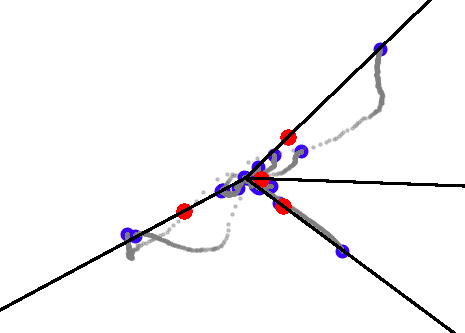
\includegraphics[height=5cm]{relu.png}
  \caption{Convergence to the global minimum}
  \label{fig:sub3}
\end{subfigure}%
\begin{subfigure}{.5\textwidth}
  \centering
  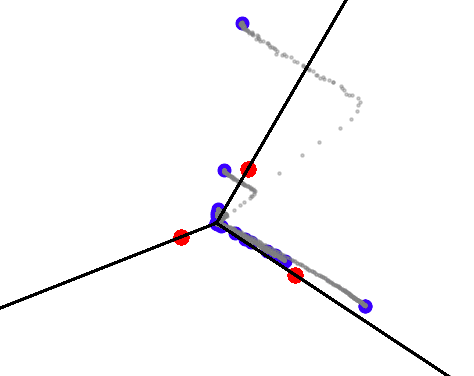
\includegraphics[height=5cm]{relu_fail.png}
  \caption{Convergence to a local minimum}
  \label{fig:sub4}
\end{subfigure}%
  \caption{Trajectories of weights during training in two different experiments with ReLU}
\end{figure}


In the case of sigmoid activations functions, we make the same experiment, except that the data is distributed on a fixed sphere in $\mathbb{R}^2$. The trained network is initialized with $w(0)=0$ (in the output layer) to satisfy the separation condition.

Each particle is represented (see figure 2) by a position $v(t) \in \mathbb{R}^2$ (without the bias) and a size proportional to $|w(t)|$, in blue for $w(t)<0$ and in red for $w(t) \geq 0$. The generative network has 2 hidden units which directions are displayed as solid black lines. 


\begin{figure}[h]
\centering
\begin{subfigure}{.5\textwidth}
  \centering
  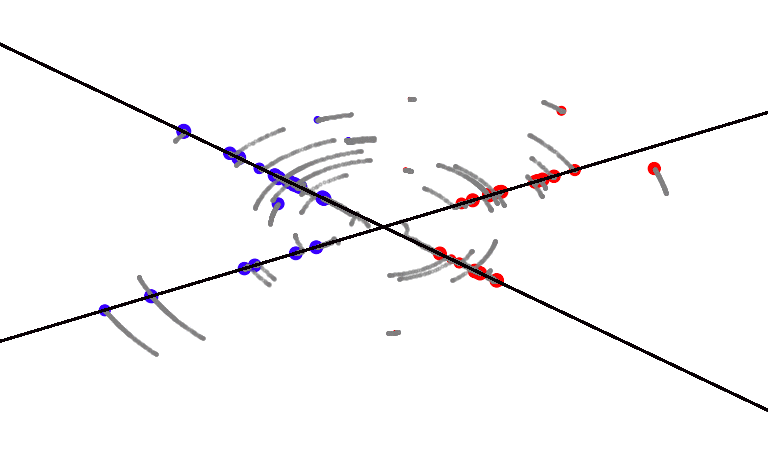
\includegraphics[width=7cm]{sig50.png}
  \caption{Convergence with 50 particles}
  \label{fig:sub3}
\end{subfigure}%
\begin{subfigure}{.5\textwidth}
  \centering
  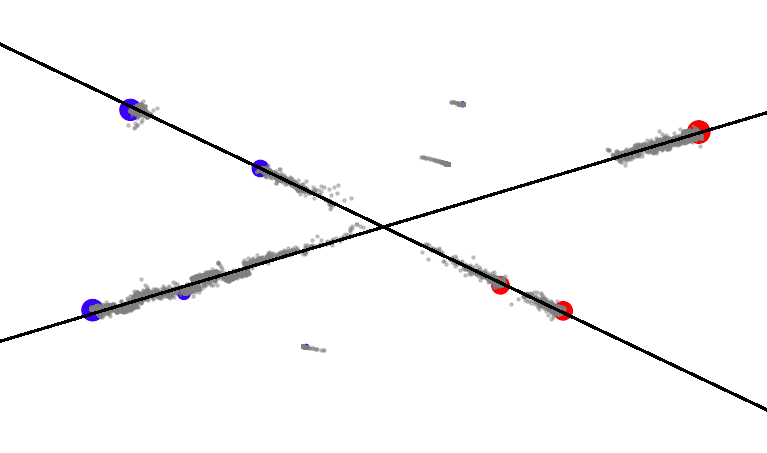
\includegraphics[width=7cm]{sig10.png}
  \caption{Convergence with 10 particles}
  \label{fig:sub4}
\end{subfigure}%
  \caption{Trajectories of weights during training with sigmoid}
\end{figure}


\subsubsection*{Observations}

For the ReLU experiment, the most decisive factor to get global convergence is the initialization of weights. The initial weights of each particle are normally distributed around zero, and then rescaled to a fixed norm $r_0$. The norm of the weights for each particle of the generative network are set to $r$. When $r_0 \ll r$, we often get global convergence. In figure 1, $r = 2$ and $r_0 = 0.05$. At initialization, all particles are located at the center and quickly get out during the first training steps. When $r_0$ in not small compared to $r$, we always obtained poor results. We will discuss more this remark in section 5.3.

Even when $r_0 \ll r$, the weights sometimes converge to a local minimum (see figure 1.b). This does not seem to be related to a lack of overparametrization, as in both experiments we considered 15 particles. In fact, the number of particles alone had little effect in this experiment to explain whether there was global convergence or not. It might only be related to the relative difficulty of some generative network configurations which may require much more particles.\\

For the sigmoid experiment, we noticed that the initialization of all output layer weights $w$ to 0 brings some separation of the particles at the beginning of training. Roughly half of them get negative weights and the other half positive weights, and this does not change through training.

In our experiment the generative network had 2 hidden units. We always got convergence to the global minimum: all particles are on the black lines, and those that are not have an output weight $w$ vanishing to zero (see the small particles in the middle of figures 2.a and 2.b).


Global convergence was obtained even with as few as 3 particles. Yet the amount of overparametrization seems to influence stability during training. When there are many particles, the weights move slower and smoother than with just a few particles (see the difference between figures 2.a and 2.b). This motivates a more careful study of the amount of overparametrization needed to achieve global convergence in section 5.2.

\subsection{How much overparametrization is needed?}

In the infinite overparametrization limit, gradient descent should converge to the global minimum under proper initialization. We may wonder if this asymptotic result already has an effect for a reasonable number of particles. We can reproduce the first experiment in a more quantitative way to measure this effect. We now consider dimension $d=50$, and we generate the data with a neural network with $M=10$ hidden units.

We train a neural network with $k$ hidden units with SGD on data generated by this first network. We want to measure the value of $k$ above which we have global convergence. Since the data is generated by another one-hidden layer neural network, the global minimum of the loss is zero. We train the network (initialized in the same way as in section 5.1) with new samples at each gradient step. The train loss is computed on the rolling set of the last 1,000 training samples and is only here for illustration. The test loss is estimated on a new set of 10,000 samples.


\begin{figure}[H]
\centering
\begin{subfigure}{.5\textwidth}
  \centering
  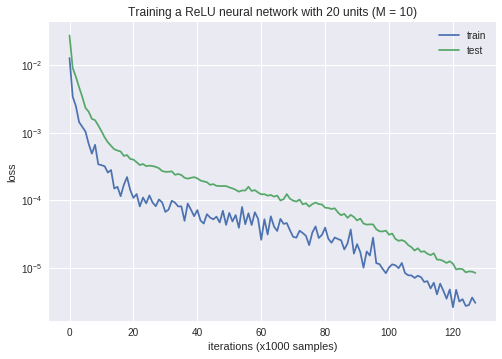
\includegraphics[width=7.5cm]{over.png}
  \caption{Convergence to zero loss with 20 particles}
  \label{fig:sub3}
\end{subfigure}%
\begin{subfigure}{.5\textwidth}
  \centering
  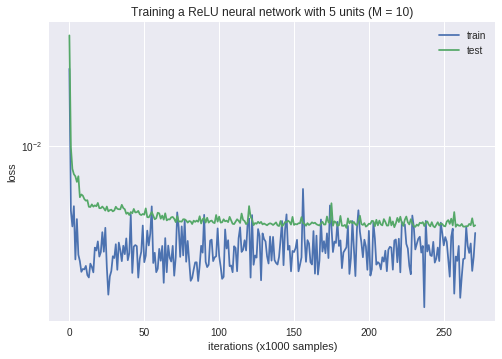
\includegraphics[width=7.5cm]{under.png}
  \caption{Convergence to non zero loss with 5 particles}
  \label{fig:sub4}
\end{subfigure}%
  \caption{Training with ReLU in overparametrization and underparametrization regimes}
\end{figure}


When $k < M$, the loss cannot converge to zero in general so it must converge to a local minimum (see figure 3.b). In the overparametrization limit (see figure 3.a), the loss converges to zero, but in practice we must stop the optimization at some point, plus the loss is only estimated through sampling, so we only get a very small test loss. \\

We repete the whole experiment (including drawing a new generative network) 5 times, for different values of $k$, both in the case of ReLU and sigmoid activation functions. We plot the geometric mean of the obtained losses for each value of $k$ in figures 4 and 5.

In the two plots we see a fall in the loss for $k$ around $M=10$. It is like a phase transition. For low values of $k$, the loss can only go to a non zero minimum and provide a solution which quality depends on the structure of the true network. For high values of $k$, optimization is slower, and since we stopped it after the same number of steps for different $k$, it might explain why the loss goes up for $k \geq 30$ in figure 4. Interestingly, in both figures 4 and 5, the excess loss has a higher variance for $k$ near the true number of particles $M$, and this variance is reduced for higher values of $k$. It could mean that we are in a regime where the convergence is more deterministic and stops depending on the generative network and on the initializations.\\

This supports the remark of \cite{chizat2018global} that only a slight overparametrization is needed to find a global minimizer, even though we did not manage to reproduce the sharp transition that they obtained in the same experiment.




\begin{figure}[H]
\centering
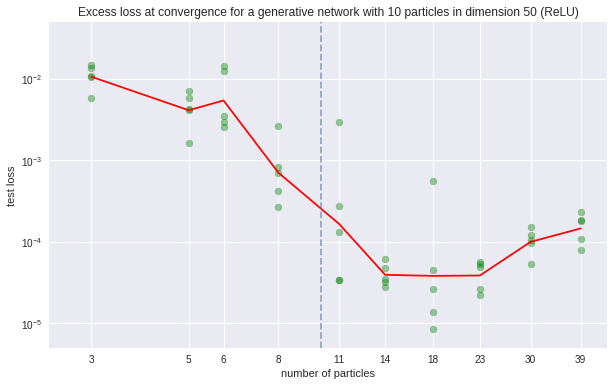
\includegraphics[width=10cm]{lossr.png}
  \caption{Excess loss at convergence for an increasing number of particles with ReLU}
  \label{fig:3}
\end{figure}

\begin{figure}[H]
\centering
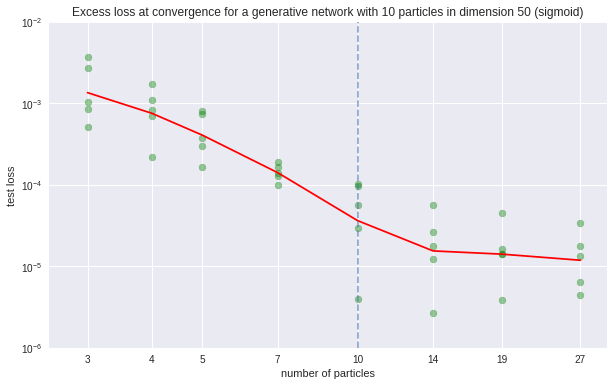
\includegraphics[width=10cm]{loss.png}
  \caption{Excess loss at convergence for an increasing number of particles with sigmoid}
  \label{fig:3}
\end{figure}


\subsection{Lazy or active training?}

In section 5.1, in the case of ReLU, we noticed that the radius of the sphere where we initialized all the particles had an influence on the convergence. Here we try to make this statement more precise. We get back to dimension 2 and generate the data with $M=3$ hidden units, with parameters on the sphere of radius $r=2$. We consider overparametrized neural networks with $k=20$ particles initialized on the sphere of radius $r_0$ and we study the influence of $r_0$.

We plot (see figure 6) the test loss during training with SGD and a fixed number of samples (500,000) and fixed learning rate. The whole experiment is repeted 5 times so we plot the geometric mean, minimum and maximum of the loss (in log scale). The best choice of $r_0$ seems to be 0.05 like in our first experiment. For a big value $r_0 = 10$, training is very slow and unstable. For $r_0$ too small, the variance between the experiments was too high to conclude anything. It might be explained by the singularity of the ReLU function around zero.

\begin{figure}[h]
\centering
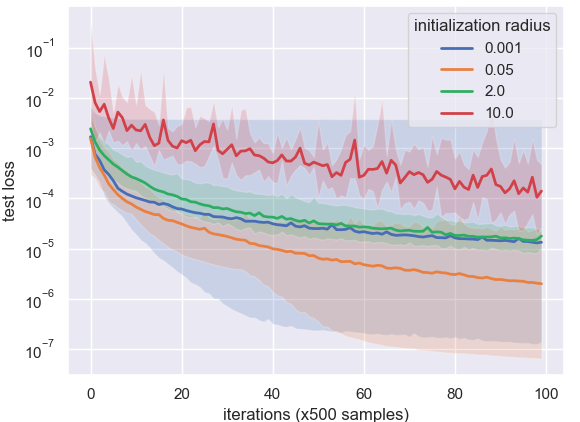
\includegraphics[width=9cm]{radius.png}
  \caption{Influence of $r_0$ through training with $k=20$ particles}
  \label{fig:3}
\end{figure}

\begin{figure}[h]
\centering
\begin{subfigure}{.5\textwidth}
  \centering
  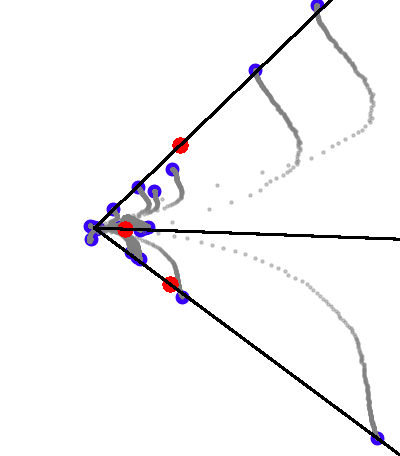
\includegraphics[height=5cm]{005.png}
  \caption{Weights trajectory for $r_0=0.05$}
  \label{fig:sub3}
\end{subfigure}%
\begin{subfigure}{.5\textwidth}
  \centering
  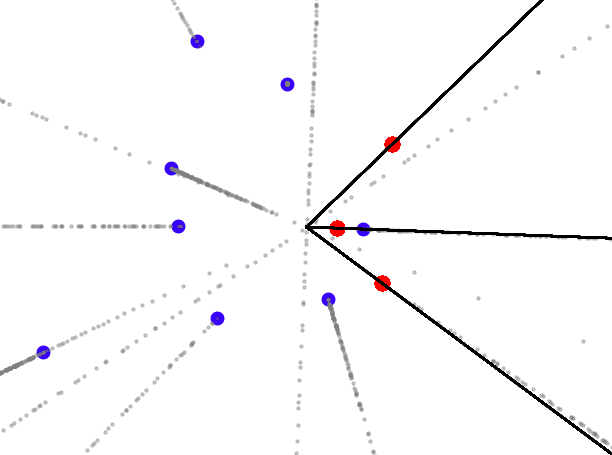
\includegraphics[height=5cm]{10.png}
  \caption{Weights trajectory for $r_0=10$}
  \label{fig:sub4}
\end{subfigure}%
  \caption{Two different behaviours in the trajectories of weights with ReLU}
\end{figure}

Getting back to the visualization in dimension 2, we can witness two very different training regimes depending on the choice of $r_0$. For small values of $r_0$ (see figure 7.a), all particles \textit{spring out} from the origin and then converge to the global optimum. For $r_0=10$, the particles only move on lines passing at the origin (see figure 7.b). It means that the only weights moving are the output weights $w_j$, and we somehow get back to the convex optimization problem with $L^2$ regularization: sampling many random hidden units and training only the output weights, which proved to be limited.\\



These observations are related, but not identical to the ones recently made by  \cite{chizat:hal-01945578}. They explain several recent results on global convergence of overparametrized neural networks by an implicit choice in the scaling of some parameters of the networks. Some conditions on this scaling lead to a particular training regime that they call \textit{lazy training}. In this case all the weights of the model stay close to their initialization, so that we can get strong convergence guarantees. But these models do not generalize well. Obviously, this is not what happens when we usually train a neural network.

In particular, they illustrate this phenomenon with one-hidden layer ReLU neural networks, by changing the variance of the initial normal distribution of weights. When the variance is high, all weights stay almost fixed. When it is low, the weights move and the model generalizes well.


\section{Conclusion}

Convex neural networks is a way to formulate the learning process of an overparametrized one-hidden layer neural network as a convex problem. It trades a non convex problem in finite dimension for a convex problem in infinite dimension. When the model is properly constrained, that is, when we set an $L^1$ norm constraint on the output weights, then the number of hidden units with non zero weight is finite. This model has good generalization properties, and in particular its sample complexity has a good scaling with the dimension.

However, optimizing in infinite dimension is hard in general. A natural choice of algorithm for this kind of constrained problems is conditional gradient. It turns out that in the case of convex neural networks, the subproblem of adding a new hidden unit is provably NP-hard for standard choices of activation functions. Hence solving the training problem of convex neural networks with exact conditional gradient is intractable. Whether there exists a polynomial time approximation to this subproblem preserving the generalization bounds is still an open question.

We may consider another approach to efficiently optimize neural networks. Gradient descent can be seen as a continuous time process in the space of measures. Results from optimal transport provide global optimality guarantees for gradient descent in the overparametrization limit, under initialization and homogeneity conditions. The number of hidden units needed to reach this asymptotic result and the influence of the initialization can be estimated empirically. There still lacks theoretical results quantifying this behaviour, and more generally, all the results on one-hidden layer neural networks are far from covering the variety of models used in practice.

\newpage

\bibliographystyle{apalike}
\bibliography{biblio.bib}

 




\end{document}
